\documentclass[a4paper]{article}
\usepackage[utf8]{inputenc}
\usepackage{lmodern}
\usepackage[T1]{fontenc}
\usepackage[italian]{babel}
\usepackage{microtype}
\usepackage{acronym}
\usepackage{mathtools}
\usepackage{amsfonts}
\usepackage{amsthm}
\usepackage[hidelinks,breaklinks=true]{hyperref}
\usepackage{xcolor}
\usepackage{listings}

\newcommand{\me}{\ensuremath{\mathrm{e}}}
\newcommand{\md}{\ensuremath{\mathrm{d}}}
\newcommand{\tc}{\ensuremath{\mathrm{t.c.:}\quad}}
\newcommand{\expected}[1]{\ensuremath{\mathrm{\textbf{E}}\left[#1\right]}}
\newcommand{\variance}[1]{\ensuremath{\mathrm{\textbf{Var}}\left(#1\right)}}
\newcommand{\prob}[1]{\ensuremath{\mathrm{\textbf{P}}\left(#1\right)}}
%\newcommand{\max}[1]{\ensuremath{\mathrm{max}\left(#1\right)}}
\newcommand{\abs}[1]{\ensuremath{\left|#1\right|}}
\newcommand{\mR}{\ensuremath{\mathbb{R}}}
\newcommand{\codei}[1]{\texttt{#1}}

%\newtheorem{defi}{Definizione}[chapter]

\lstset{inputpath=src}
\lstdefinestyle{customPy}{
 language=python,
 showstringspaces=false,
 basicstyle=\footnotesize\ttfamily,
 keywordstyle=\bfseries\color{green!40!black},
 commentstyle=\itshape\color{purple!40!black},
 identifierstyle=\color{blue},
 stringstyle=\color{orange},
}

%\DeclarePairedDelimiter\abs{\lvert}{\rvert}

\author{
  {\Large Stefano Martina}\\
  {\small stefano.martina@stud.unifi.it}\\
  Universit\`a degli Studi di Firenze\\
  Scuola di Scienze Matematiche, Fisiche e Naturali\\
  Corso magistrale di Informatica
}
\title{{\Huge\bfseries A simulated annealing approach to solve path
    planning}}%\\{\large\bfseries Esame di Laboratorio di Fisica Computazionale}}

\begin{document}
\maketitle
\thispagestyle{empty}
\vfill
\begin{abstract}
  This work is about a simulated annealing method for performing path
  planning.
\end{abstract}

\section{Introduction}
The \emph{Path planning} problem is a common problem in robotics, the
purpose is to find the best route in a bidimensional (or
tridimensional) space with obstacles in it, from one point to
another.

\section{Path planning}
In this project the space is bidimensional and the obstacles are
represented as an array of vertexes and are closed polygons - the last
vertex is connected to the first one. The path is calculated from a
provided point to another provided point in the space, and is assumed
that the user don't choose one or both of those points inside an
obstacle.

Is also possible - and adviced - to add a bounding box around the
scene.

The path planning is performed doing a simulated annealing using, as the state of the system, the
configuration of the vertexes of the path; a Dijkstra algorithm is
performed for finding the initial state of the system, using a pruned 
Voronoi diagram as basis.

\section{Algorithm}
Initially the algorithm distribute a series of points along the edges
of the obstacles and the bounding box, then build a Voronoi diagram
using that points as
input sites. After that transform the diagram in a graph, using the
vertexes and edges of the cells as nodes and edges of the graph, then
delete all the edges that cross an obstacle. The result is a sparse
graph that embrace all obstacles and that maintain equal distance from
obstacles, like in image~\ref{fig:voronoi}
\begin{figure}[htb]
  \centering
  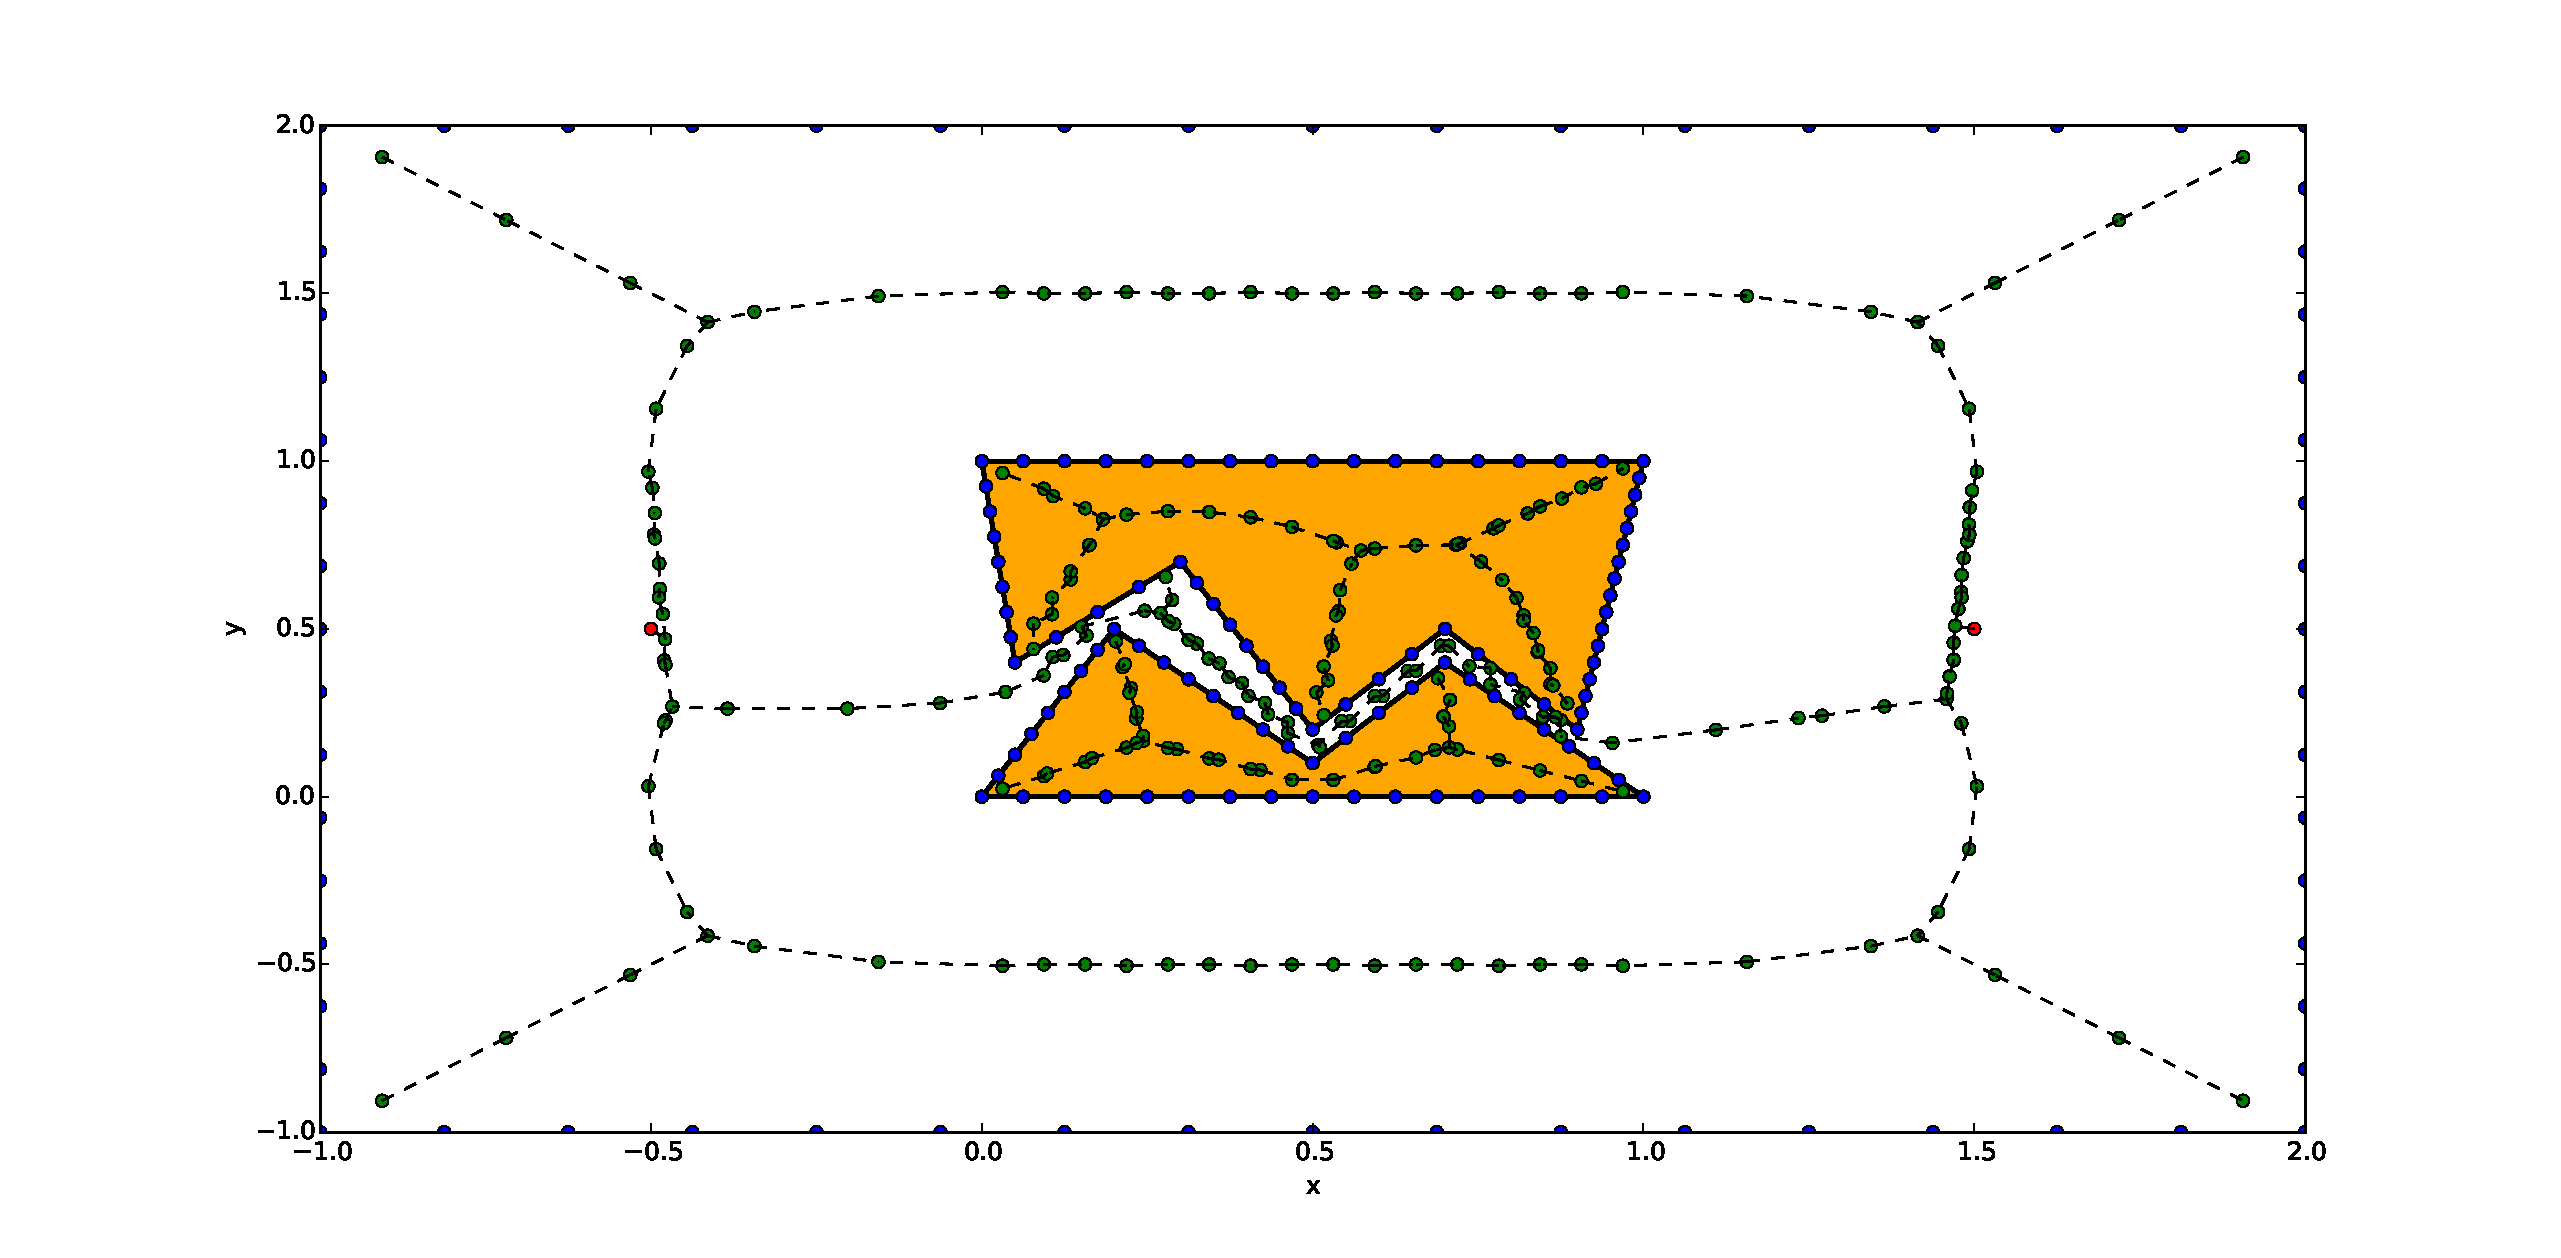
\includegraphics[width=\textwidth]{img/voronoi.pdf}
  \caption{Pruned Voronoi graph}
  \label{fig:voronoi}
\end{figure}

\section{Conclusions}

\end{document}

